\documentclass{article}

\usepackage[ngerman]{babel}
\usepackage{graphicx}
\usepackage{indentfirst}
\usepackage{hyperref}
\usepackage{geometry}
\usepackage{changepage}
\usepackage{booktabs}
\usepackage{float}
\usepackage{tabulary}
\usepackage{multirow}

\graphicspath{ {./images/} }
\setlength\parindent{0pt}

\makeatletter
\newcommand{\sectionauthor}[1]{
	{\parindent 0em \large \scshape Autor: #1 \par \nobreak \vspace*{1em}}
	\@afterheading
}
\newcommand{\specification}[3]{
	{\parindent 0.5em \hangindent 3em \hypertarget{spec:#1:#2}{\textbf{/#1#2/}} #3 \par \nobreak \vspace*{0.5em}}
}
\makeatother

\title{Bibliotheksanwendung - Feinspezifikation}
\date{\today\\v1.0}
\author{
	Ivan Charviakou\\
	León Liehr\\
	Mohamad Najjar\\
	Jonas Picker\\
	Sergei Pravdin
}

\begin{document}
\maketitle
\begin{figure}[h]
	\centering
	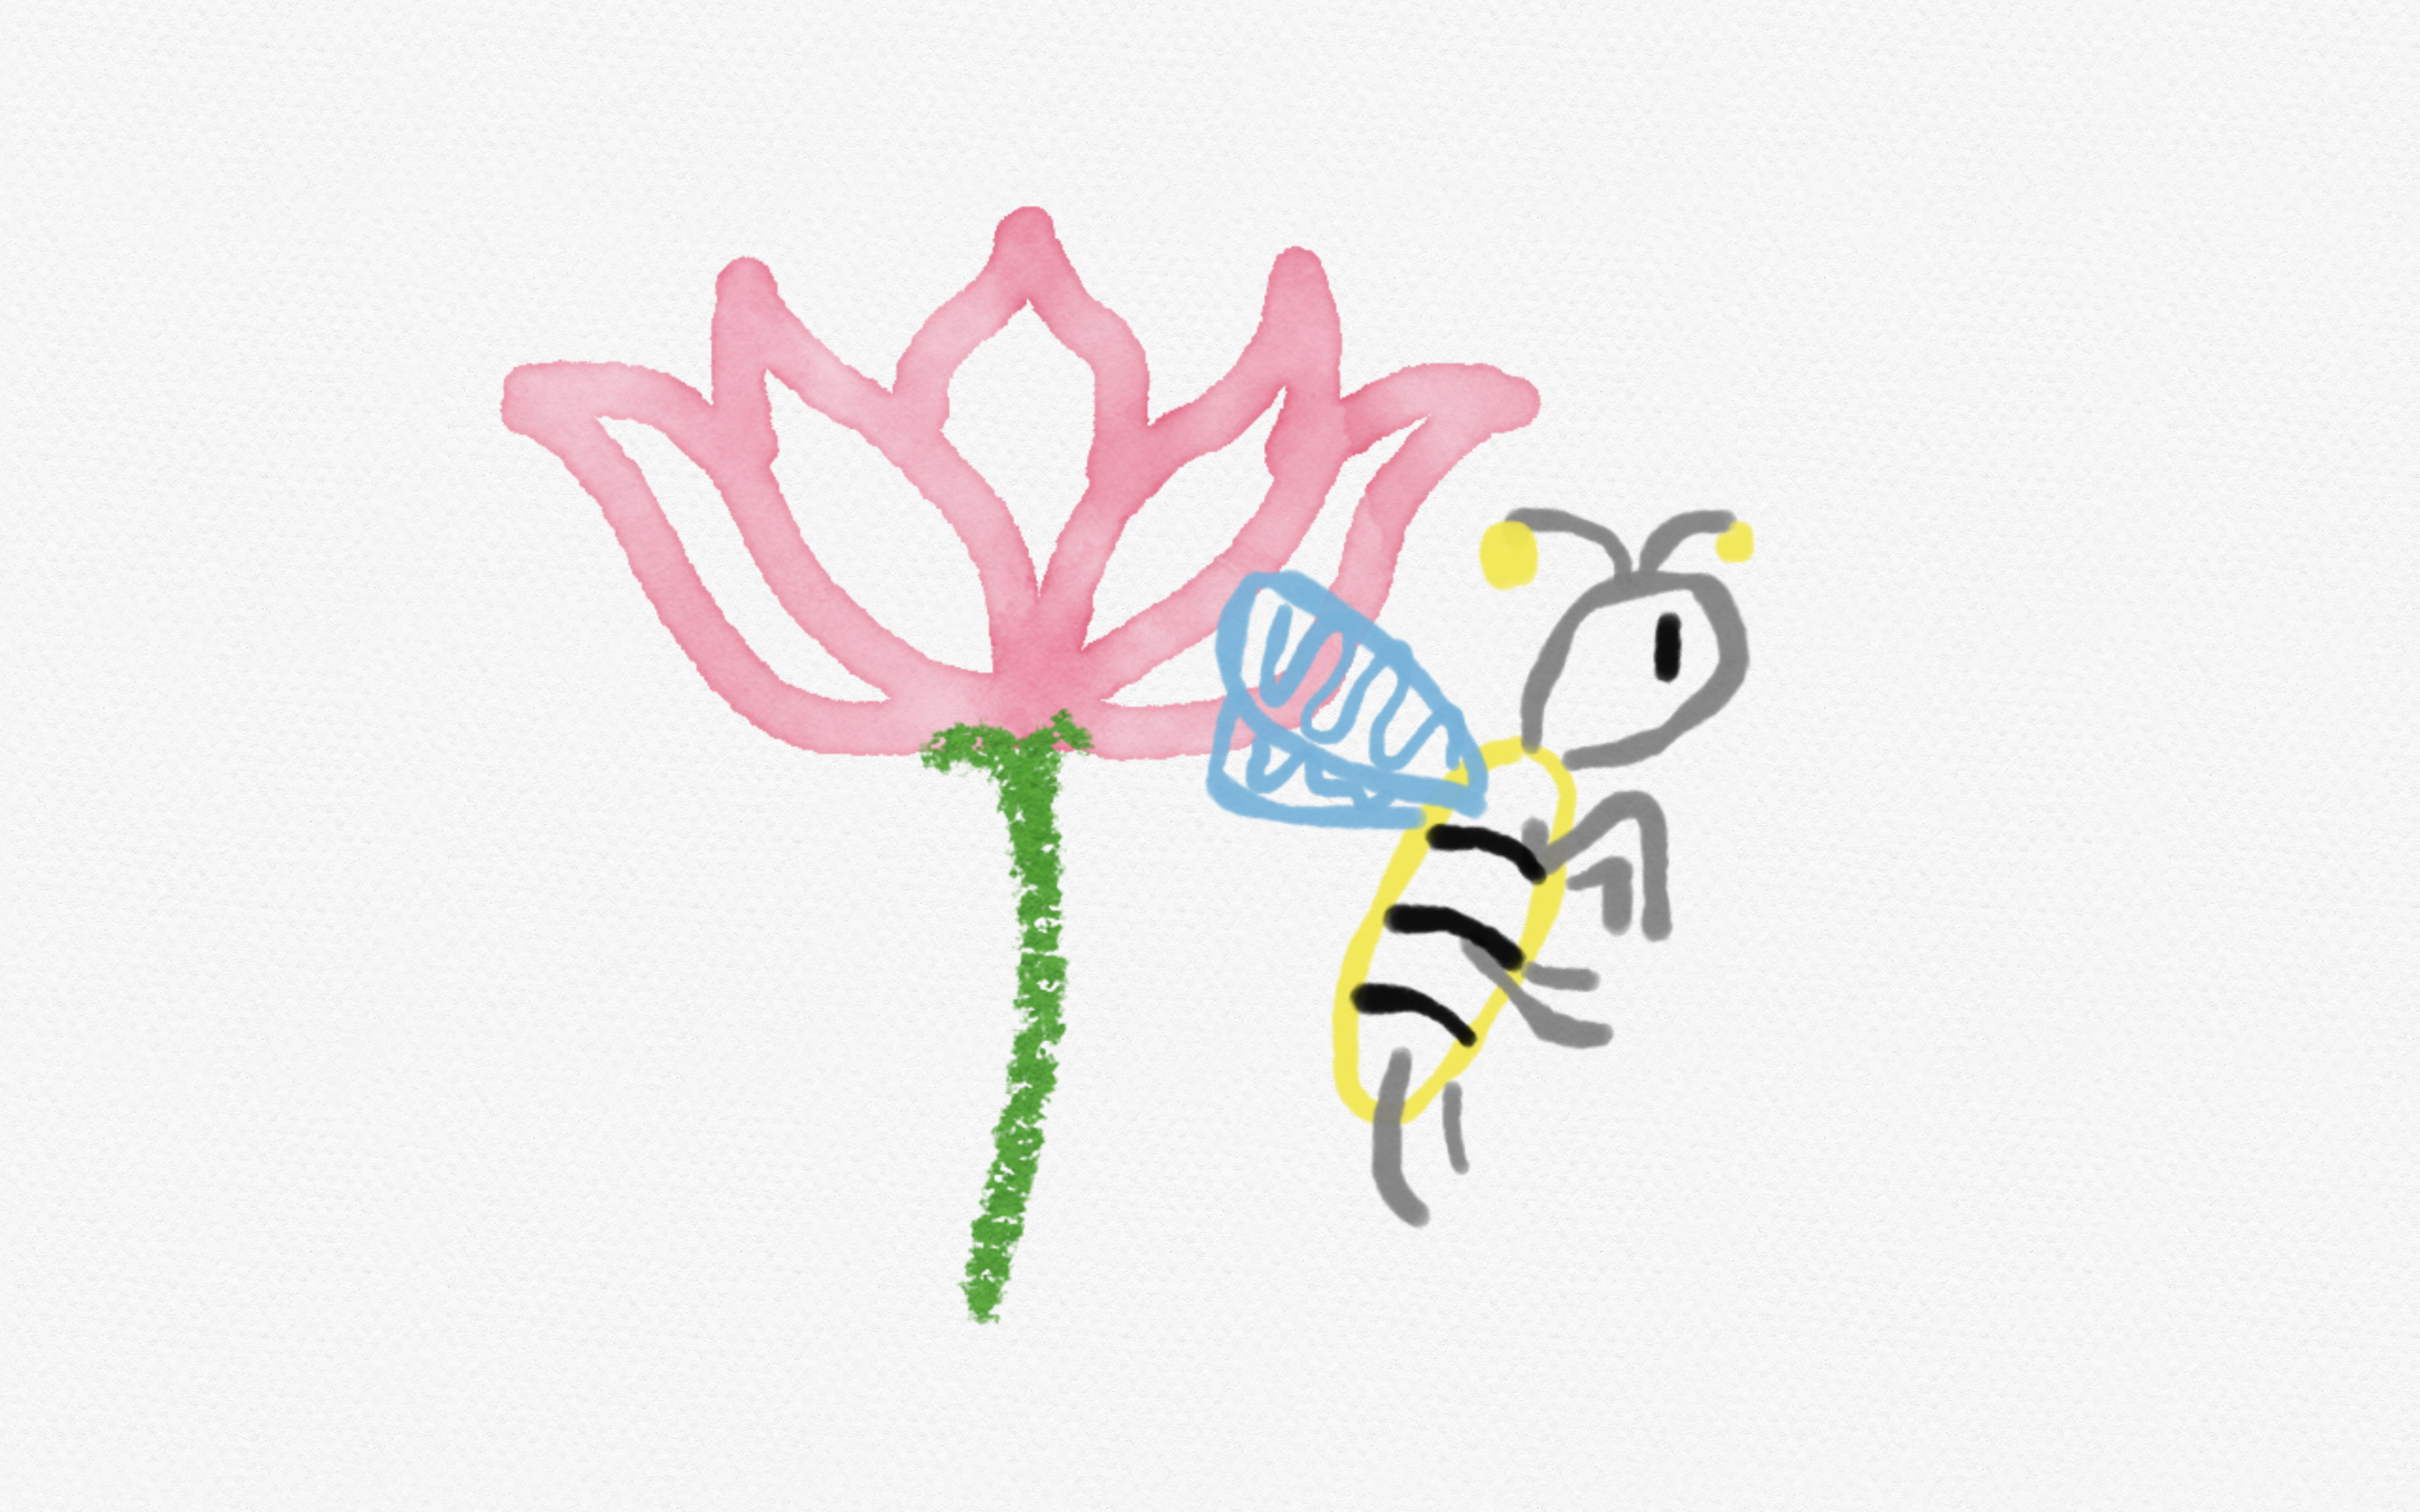
\includegraphics[width = 30em]{Logo}
\end{figure}
\newpage
\tableofcontents
\newpage

%----------------------------------------------------------------------Kapitel 1--------------------------------------------------------------------------------------------

\section{Einleitung}
Bei diesem Dokument handelt es sich um die Feinspezifikation unseres Bibliothekssystems. Es baut direkt auf dem vorangegangenen Entwurf auf und enthält einen noch genaueren Umriss der zu erstellenden Applikation.

%----------------------------------------------------------------------Kapitel 2--------------------------------------------------------------------------------------------

\section{Projektübersicht}
\sectionauthor{Ivan Charviakou}

\subsection{Paketübersicht und Ordnerstruktur}
Das angegebene Diagramm stellt die MVC-Architektur mit den Beziehungen zwischen den einzelnen Komponenten anhand der gegebenen Applikation dar. 
Dabei folgt die Komponentenaufteilung der Paketstruktur der Applikation und es werden die Paketnamen zusammen mit den wichtigsten darin enthaltenen Klassen / Komponenten / Funktionalitäten angegeben. 
Zudem entsprechen die Farben, die die Pakete im Diagramm besitzen, den Farben im nachfolgenden Klassendiagramm. \vspace{0.5em}

Die Ordnerstruktur des Projekts wird als Ordnerbaum dargestellt. 
Während die Paketstruktur im Ordner 'BiBi.src.main.java' abgebildet ist, enthält 'BiBi.src.main.webapp.view' die verwendeten Facelets mit entsprechender Rollenzuordnung. \vspace{0.5em}

\begin{figure}[h]

\end{figure}

\begin{figure}[h]
	\centering
	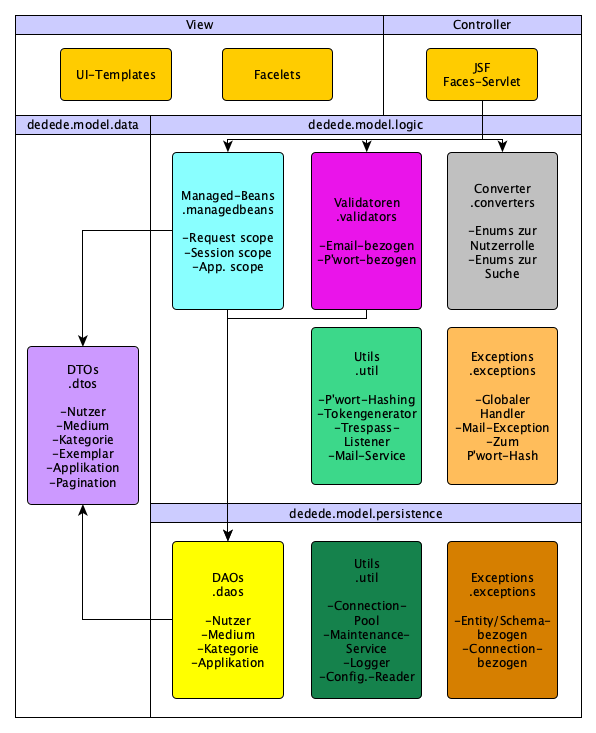
\includegraphics[width = 20em]{Modeldiagramm}
\end{figure}
\begin{figure}[h]
	\centering
	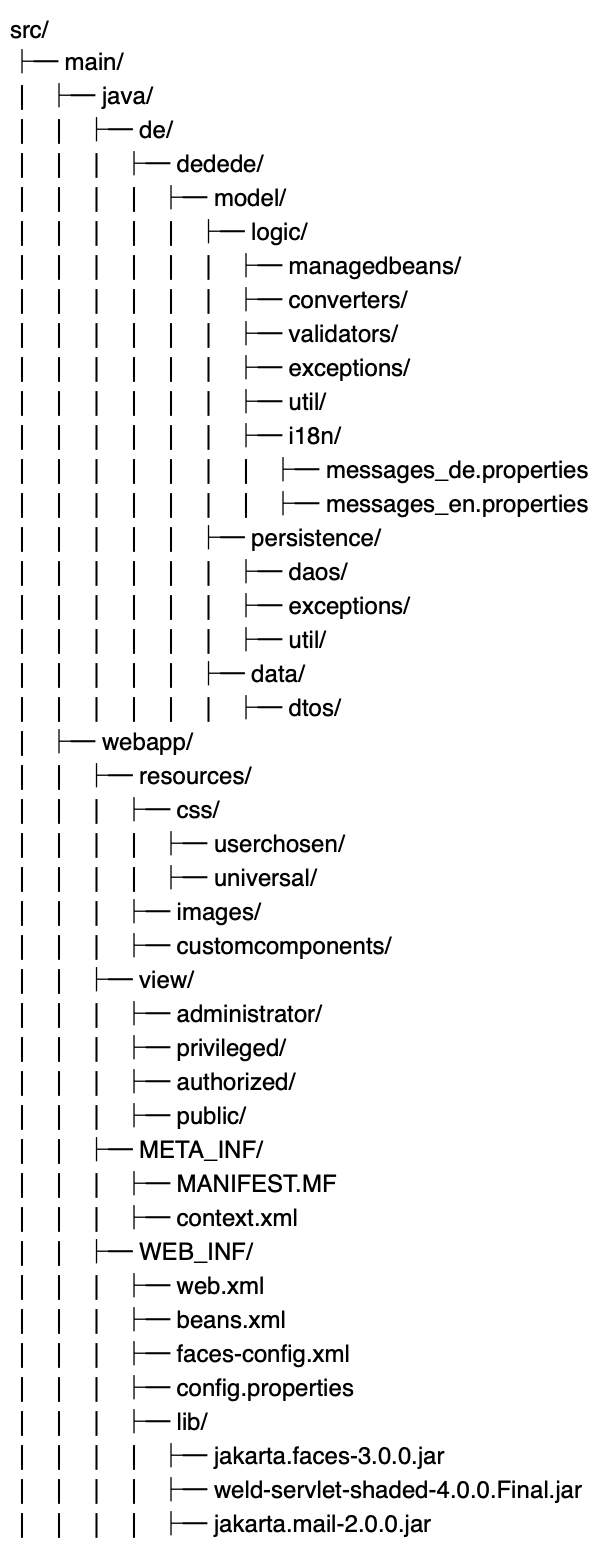
\includegraphics[width = 15em]{FileStructure}
\end{figure}

%----------------------------------------------------------------------Kapitel 3--------------------------------------------------------------------------------------------


%----------------------------------------------------------------------Kapitel 4--------------------------------------------------------------------------------------------
\newpage
\section{Bibliotheken}
\sectionauthor{Sergei Pravdin}

\newenvironment{controls}
{
    \begin{table}[H]
        \centering
        \begin{tabular}{ p{7em} p{19em} p{4em} p{12em} }
            \toprule
            \textbf{Bibliothek} & \textbf{Anwendungsbereich} & \textbf{Version} & \textbf{Lizenz}\\
            \midrule
        }
        {
            \bottomrule
        \end{tabular}
    \end{table}
}

Folgende Bibliotheken bzw. Frameworks werden für die Entwicklung unseres Bibliothekssystems verwendet.

\begin{controls}
    Jakarta Server Faces (JSF) & Grafische Benutzeroberflächen des Bibliothekssystems & 3.0.0 & GNU GPL / Java Community Process\\
    JDBC-Treiber für PostgreSQL & Integration des Bibliothekssystems mit der Datenbank & 42.2.20 & GNU GPL / Java Community Process\\
    Apache Tomcat & Webserver & 10.0.2 & Apache-Lizenz 2.0\\
    Weld & Dependency Injection mittels Annotationen & 4.0.1 & Apache-Lizenz 2.0\\
    Jakarta Mail & Senden und Empfangen von E-Mails für die Verifizierung der Nutzers & 1.6.5 & CDDL 1.0, GPL 2.0, BSD\\
    Bootstrap & Anordnung der Frontend-CSS-Komponenten & 5.0.0 & MIT-Lizenz\\
\end{controls}

%----------------------------------------------------------------------Kapitel 5--------------------------------------------------------------------------------------------


%----------------------------------------------------------------------Kapitel 6--------------------------------------------------------------------------------------------


%----------------------------------------------------------------------Kapitel 7--------------------------------------------------------------------------------------------


%----------------------------------------------------------------------Kapitel 8--------------------------------------------------------------------------------------------
\newpage
\section{Datenfluss}
\sectionauthor{Sergei Pravdin}
Die Kommunikation zwischen den Klassen und die Interaktionen des Systems werden durch die Sequenzdiagramme abgebildet. Um einen Datenfluss beispielhaft zu zeigen, werden die folgenden beiden Szenarien vorgelegt: Zuerst bucht ein angemeldeter Nutzer ein Medium-Exemplar erfolgreich zur Ausleihe. Im zweiten Szenario bucht ein angemeldeter Nutzer ein Medium-Exemplar erfolglos zur Ausleihe, weil die Verbindung mit der Datenbank fehlgeschlagen ist. Das System ist so eingestellt, dass die angemeldeten Nutzer Zugriff auf die Medien haben. Der Nutzer möchte ein Exemplar des Mediums 'Programmieren lernen' buchen. Im System existiert das Medium mit dem Titel 'Programmieren lernen' und mit der Signatur (ID) '17RE'. Das Exemplar mit der Signatur (ID) '17RE (+1)' gehört zu dem genannten Medium und ist für eine Buchung verfügbar. Der Nutzer ruft die Mediumsseite 'medium.xhtml?id=17RE' auf.
\subsection{Interaktionen beim erfolgreichen Buchen eines Medium-Exemplars}
\subsubsection{Initialisierung der Mediumsseite}
Beim Laden der Mediumsseite wird zuerst die Methode 'init' als @PostConstruct aufgerufen. Die 'init'-Methode erzeugt ein Medium-DTO, das Medium-DTO hat eine Kollektion der CopyDTOs und eine Kollektion der AttributeDTOs, folglich werden sie vom Medium-DTO erstellt. Der Nutzer bekommt das MediumDTO und setzt eine Medium-ID, die aus dem 'viewParam' zur Verfügung gestellt wird. Danach wird die 'viewAction()' durchgeführt, welche die Mediumsseite durch die statische Methode aus dem Medium-DAO liefern muss. Das Medium-DAO bekommt auf der Persistence-Schicht eine Verbindung von der Singleton-ConnectionPool-Klasse durch die Methoden 'getInstance()' und 'getConnection()'. Im Körper der Methode 'loadMedium' wird eine SELECT-Anfrage durchgeführt, danach gibt das Medium-DAO die Verbindung durch die Methode 'releaseConnection' frei. Das Medium-DAO befüllt mit den von der Datenbank erhaltenen Attributen das Medium-DTO (inkl. CopyDTOs und AttributeDTOs) und gibt es dem Medium-BB zurück. Die Mediumsseite ist nun durch die Methode 'getAttributes' des Medium-DTOs vollständig geladen.
\subsubsection{Buchen eines Exemplars}
Durch die Methode 'getCopies' des Medium-DTOs ist das gewünschte Exemplar für den Nutzer sichtbar. Der Nutzer klickt auf den Buchen-Button des Exemplars. Beim Klicken ruft der Nutzer die Methode 'pickUpAnyCopy' des Medium-BBs auf. Im Körper dieser Methode wird die Methode 'checkAccountStatus()' aus dem UserSession-BB aufgerufen, um zu prüfen, ob der Nutzer Zugriff auf die Funktion Buchen hat. Das UserSession-Bean meldet dem Medium-BB ein positives Ergebnis (OPENED-Status) zurück. Das Medium-BB ruft die statische Methode 'MediumDAO.pickUpAnyCopy(mediumDTO)' auf. Das Medium-DAO bekommt durch die Methoden 'getInstance()' und 'getConnection()' auf der Persistence-Schicht eine Verbindung von der Singleton-ConnectionPool-Klasse. Falls ein availabilityStatus des Exemplars immer noch 'AVAILABLE' ist, wird wird eine UPDATE-Anfrage im Körper der Methode 'loadMedium'  durchgeführt. Im Anschluss gibt das Medium-DAO die Verbindung durch die Methode 'releaseConnection' frei. Als Ergebnis der Methode 'pickUpAnyCopy' bekommt das Medium-BB 'true'. Das Medium-BB vergibt den neuen Status 'MARKEDTOCOLLECT' an das Exemplar. Der Nutzer bekommt eine Nachricht durch die statische Methode 'RessourceBandleHandler.getValue()' und die Buchung ist erfolgreich abgeschlossen. Vom Ressource-Bandle-Handler wird der Nutzer entsprechend benachrichtigt.
\newgeometry{left=0cm,right=0cm,top=0cm,bottom=2cm}
\newpage
\begin{figure}[h]
    \centering
    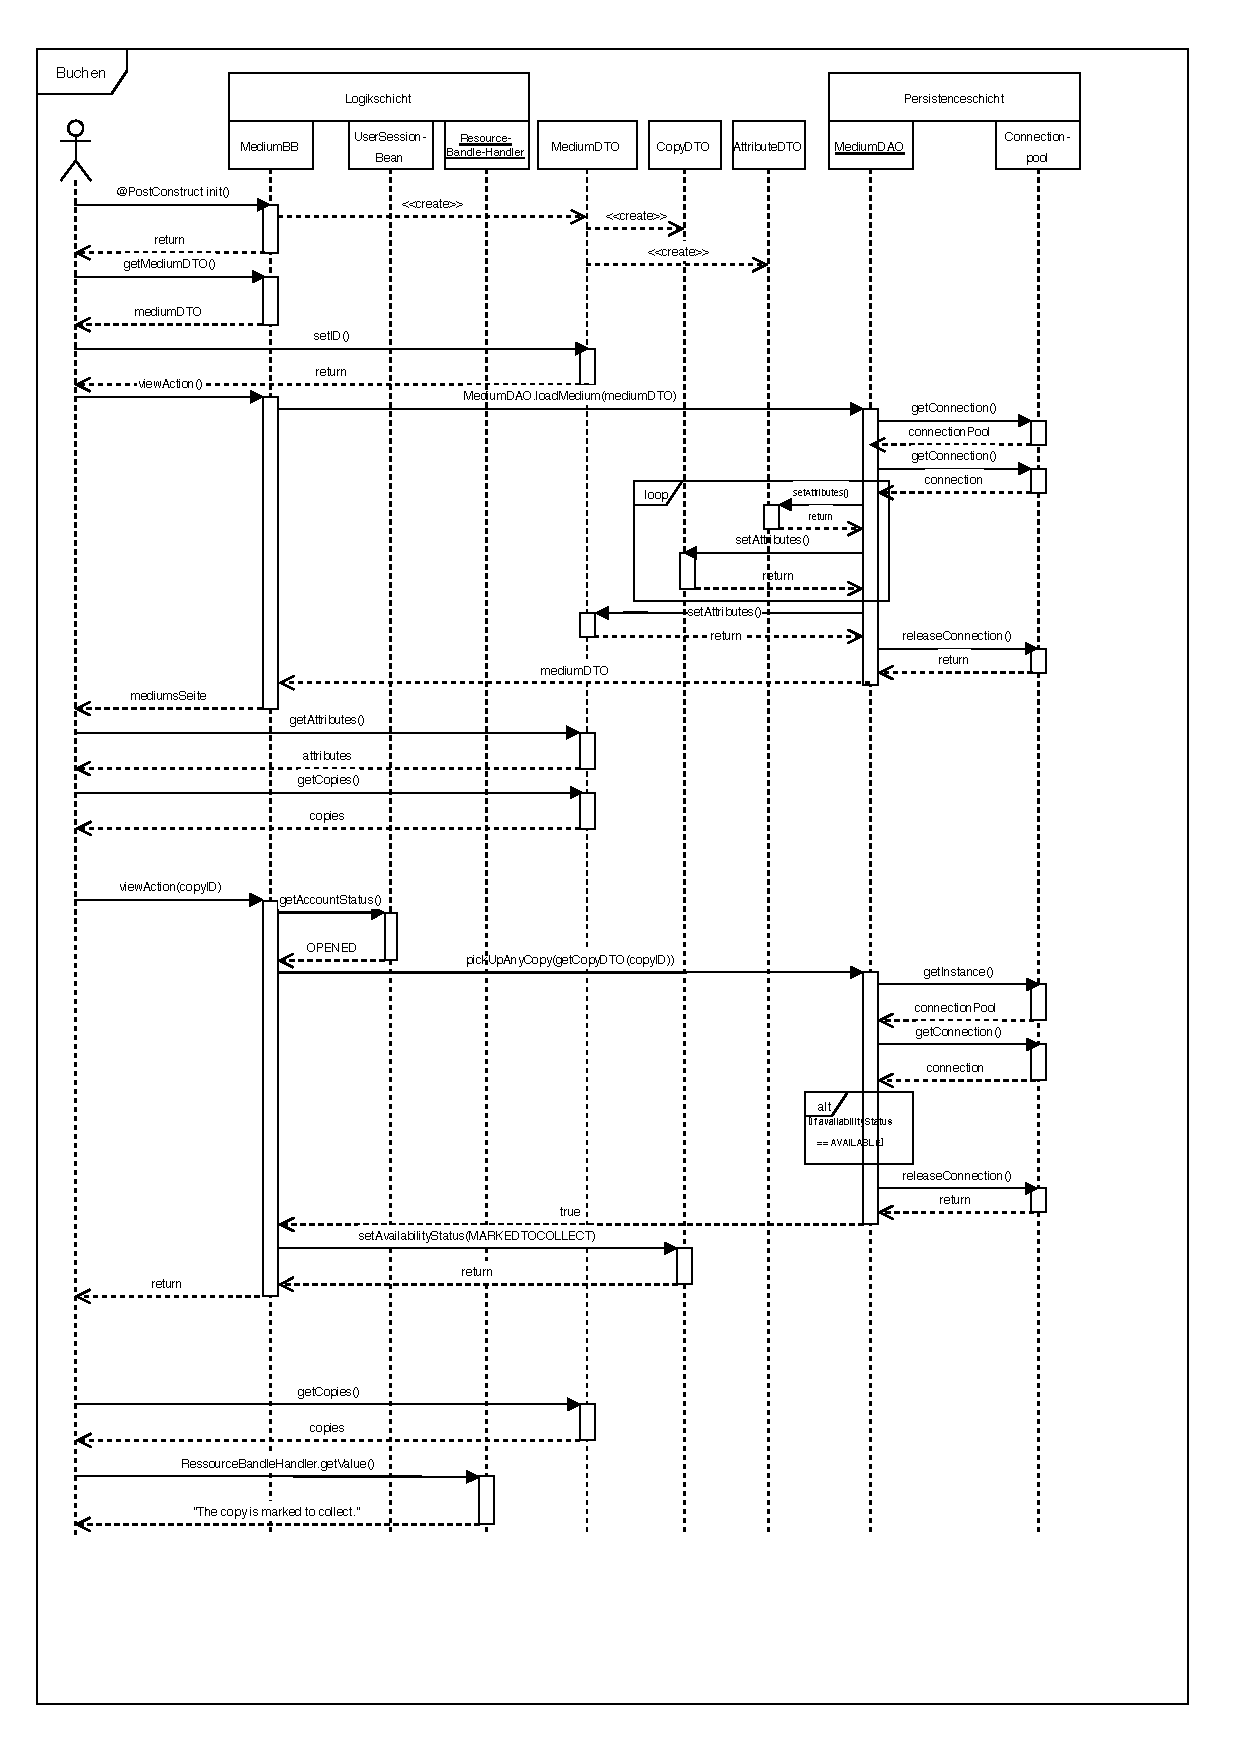
\includegraphics[width = 50em]{Sequenzdiagramm-success-v3.2}
    \caption{Interaktionen beim erfolgreichen Buchen eines Medium-Exemplars}
    \label{Sequenzdiagramm}
\end{figure}
\restoregeometry

\subsection{Interaktionen beim Buchen eines Medium-Exemplars mit fehlender Datenbankverbindung}
\subsubsection{Initialisierung der Mediumsseite}
Beim Laden der Mediumsseite wird zuerst die Methode 'init' als @PostConstruct aufgerufen. Die 'init'-Methode erzeugt ein Medium-DTO, das Medium-DTO hat eine Kollektion der CopyDTOs und eine Kollektion der AttributeDTOs, folglich werden sie vom Medium-DTO erstellt. Der Nutzer bekommt das MediumDTO und setzt eine Medium-ID, die aus dem 'viewParam' zur Verfügung gestellt wird. Danach wird die 'viewAction()' durchgeführt, welche die Mediumsseite durch die statische Methode aus dem Medium-DAO liefern muss. Das Medium-DAO bekommt durch die Methoden 'getInstance()' und 'getConnection()' auf der Persistence-Schicht eine Verbindung von der Singleton-ConnectionPool-Klasse. Aufgrund der fehlenden Verbindung mit der Datenbank kann das Medium-DAO keine SELECT-Anfrage durchführen, deshalb bekommt das Medium-DAO einen SQL-Exception. Das Medium-DAO wandelt den SQL-Exception in den DataAccess-Exception um, danach gibt das Medium-DAO eine Verbindung durch die Methode 'releaseConnection' frei. Im nächsten Schritt wirft das MediumDAO einen Data-Access-Exception in den Medium-BB ein. Der Nutzer ruft die Methode 'handle' des ExceptionHandlers auf; der ExceptionHandler gibt den Fehler durch die Methoden 'getInstance()' und 'addValue(Data-Access-Exception)' in die Singleton-Logger-Klasse ein. Danach bekommt der ExceptionHandler eine Message vom Resource-Bandle-Handler und setzt diese Message in die ErrorBB-Klasse ein. 
\subsubsection{Weiterleitung zur Fehlerseite}
Als Ergebnis der Methode 'handle' liefert der ExceptionHandler dem Nutzer den Link zur Fehlerseite. Das Laden der Fehlerseite wird auf dem Sequenzdiagramm nicht abgebildet.

\newpage

\newgeometry{left=0cm,right=0cm,top=0cm,bottom=2cm}

\begin{figure}[h]
	\hypertarget{Fehlersequenz}{}
    \centering
    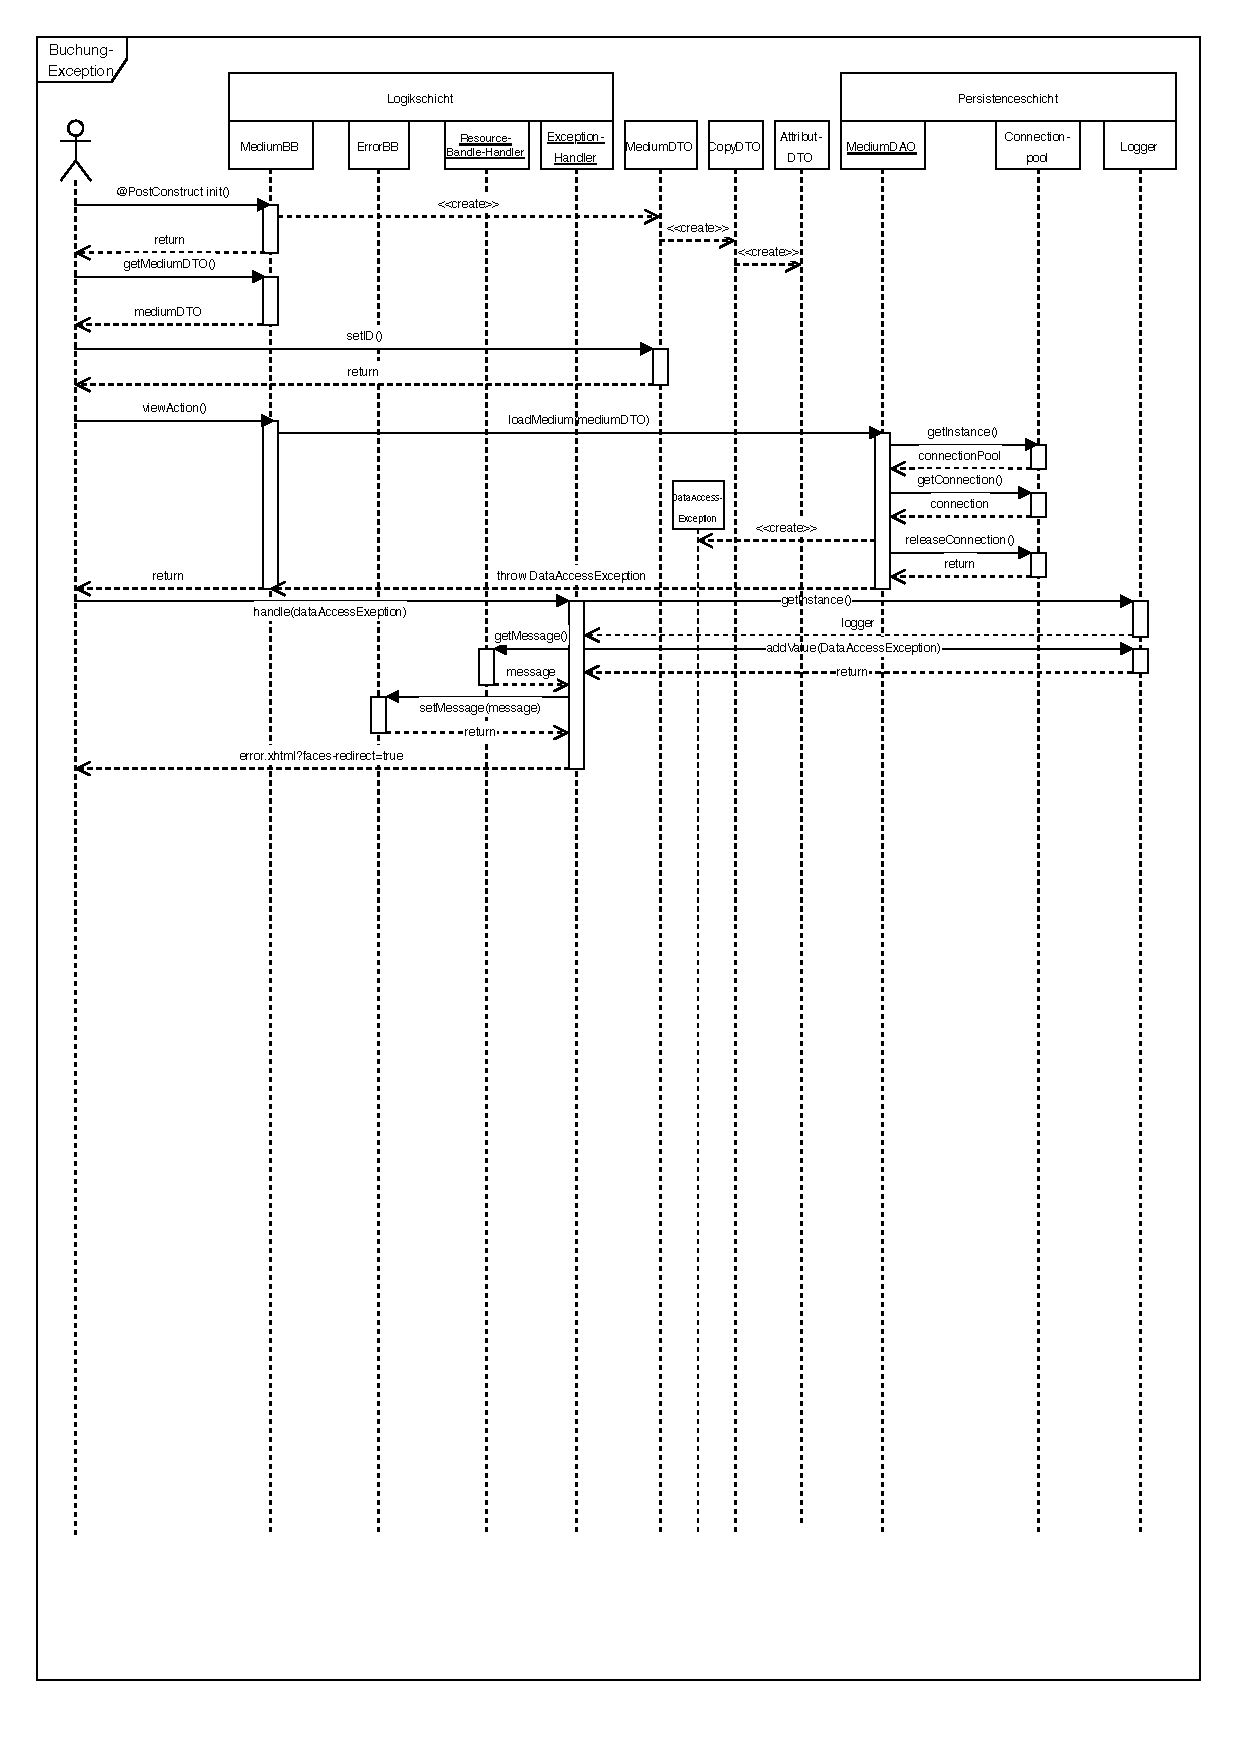
\includegraphics[width = 50em]{Sequenzdiagramm-exception-v4.1}
    \caption{Interaktionen beim Buchen eines Medium-Exemplars mit fehlender Datenbankverbindung}
    \label{Sequenzdiagramm}
\end{figure}

\restoregeometry
\newpage

%----------------------------------------------------------------------Kapitel 9--------------------------------------------------------------------------------------------


\end{document}